*** OPS! IKKE RIGTIGT! ***
This chapter creates an understanding of the given data and the different programs respectvely the program where pain maps are created and the program for development of the neural networks. 

\section{Data}
Data used in this project were collected beforehand from an on-going FOXH trial which is conducted in collaboration with Danish and Australian universities. The data consists of pain maps which were drawn by individuals with PFP through the use of an application Navigate Pain in a clinical setting. In addition to the pain maps an appurtenant dataset was available. This contained information regarding the individuals in terms of i.a. age, gender, symptom duration, pain intensity and the most prominent knee for pain. An example of a pain drawing can be seen in figure \ref{fig:kneepainmap}.

\begin{figure} [H]
\centering
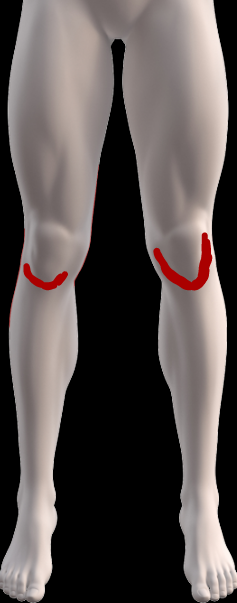
\includegraphics[width=0.25\textwidth]{figures/kneepainmap}
\caption{Pain drawings of the lower extremities. The red markings indicate the area of pain perceived by the individual subject. In this case the PFP is bilateral (on both knees).}
\label{fig:kneepainmap}
\end{figure}

\noindent
Before using the data in the deep learning model a manual data handling was necessary. This incorporate matching the given pain maps and appertaining ID regarding the individuals, which resulted in 217 pain maps. Furthermore specific information like gender, symptom duration and pain intensity is collected. The number of pain maps and associated information, gender and symptom duration, was 205. Additionally, there were 197 pain maps with associated information, gender and pain intensity.


\subsection{Software application: Navigate Pain}
Navigate Pain is a software application that is used to visualise the location, shape and spatial distribution of pain from patient to healthcare personnel. The application permits individuals to draw their pain into a body outline with different colors and line thickness. Navigate Pain android was developed at Aalborg University and a commercial web application is available at Aglance Solutions (Denmark).\citep{Solutions2015}
\autoref{fig:Navigatepain} illustrate the process using the application.

\begin{figure} [H]
\centering
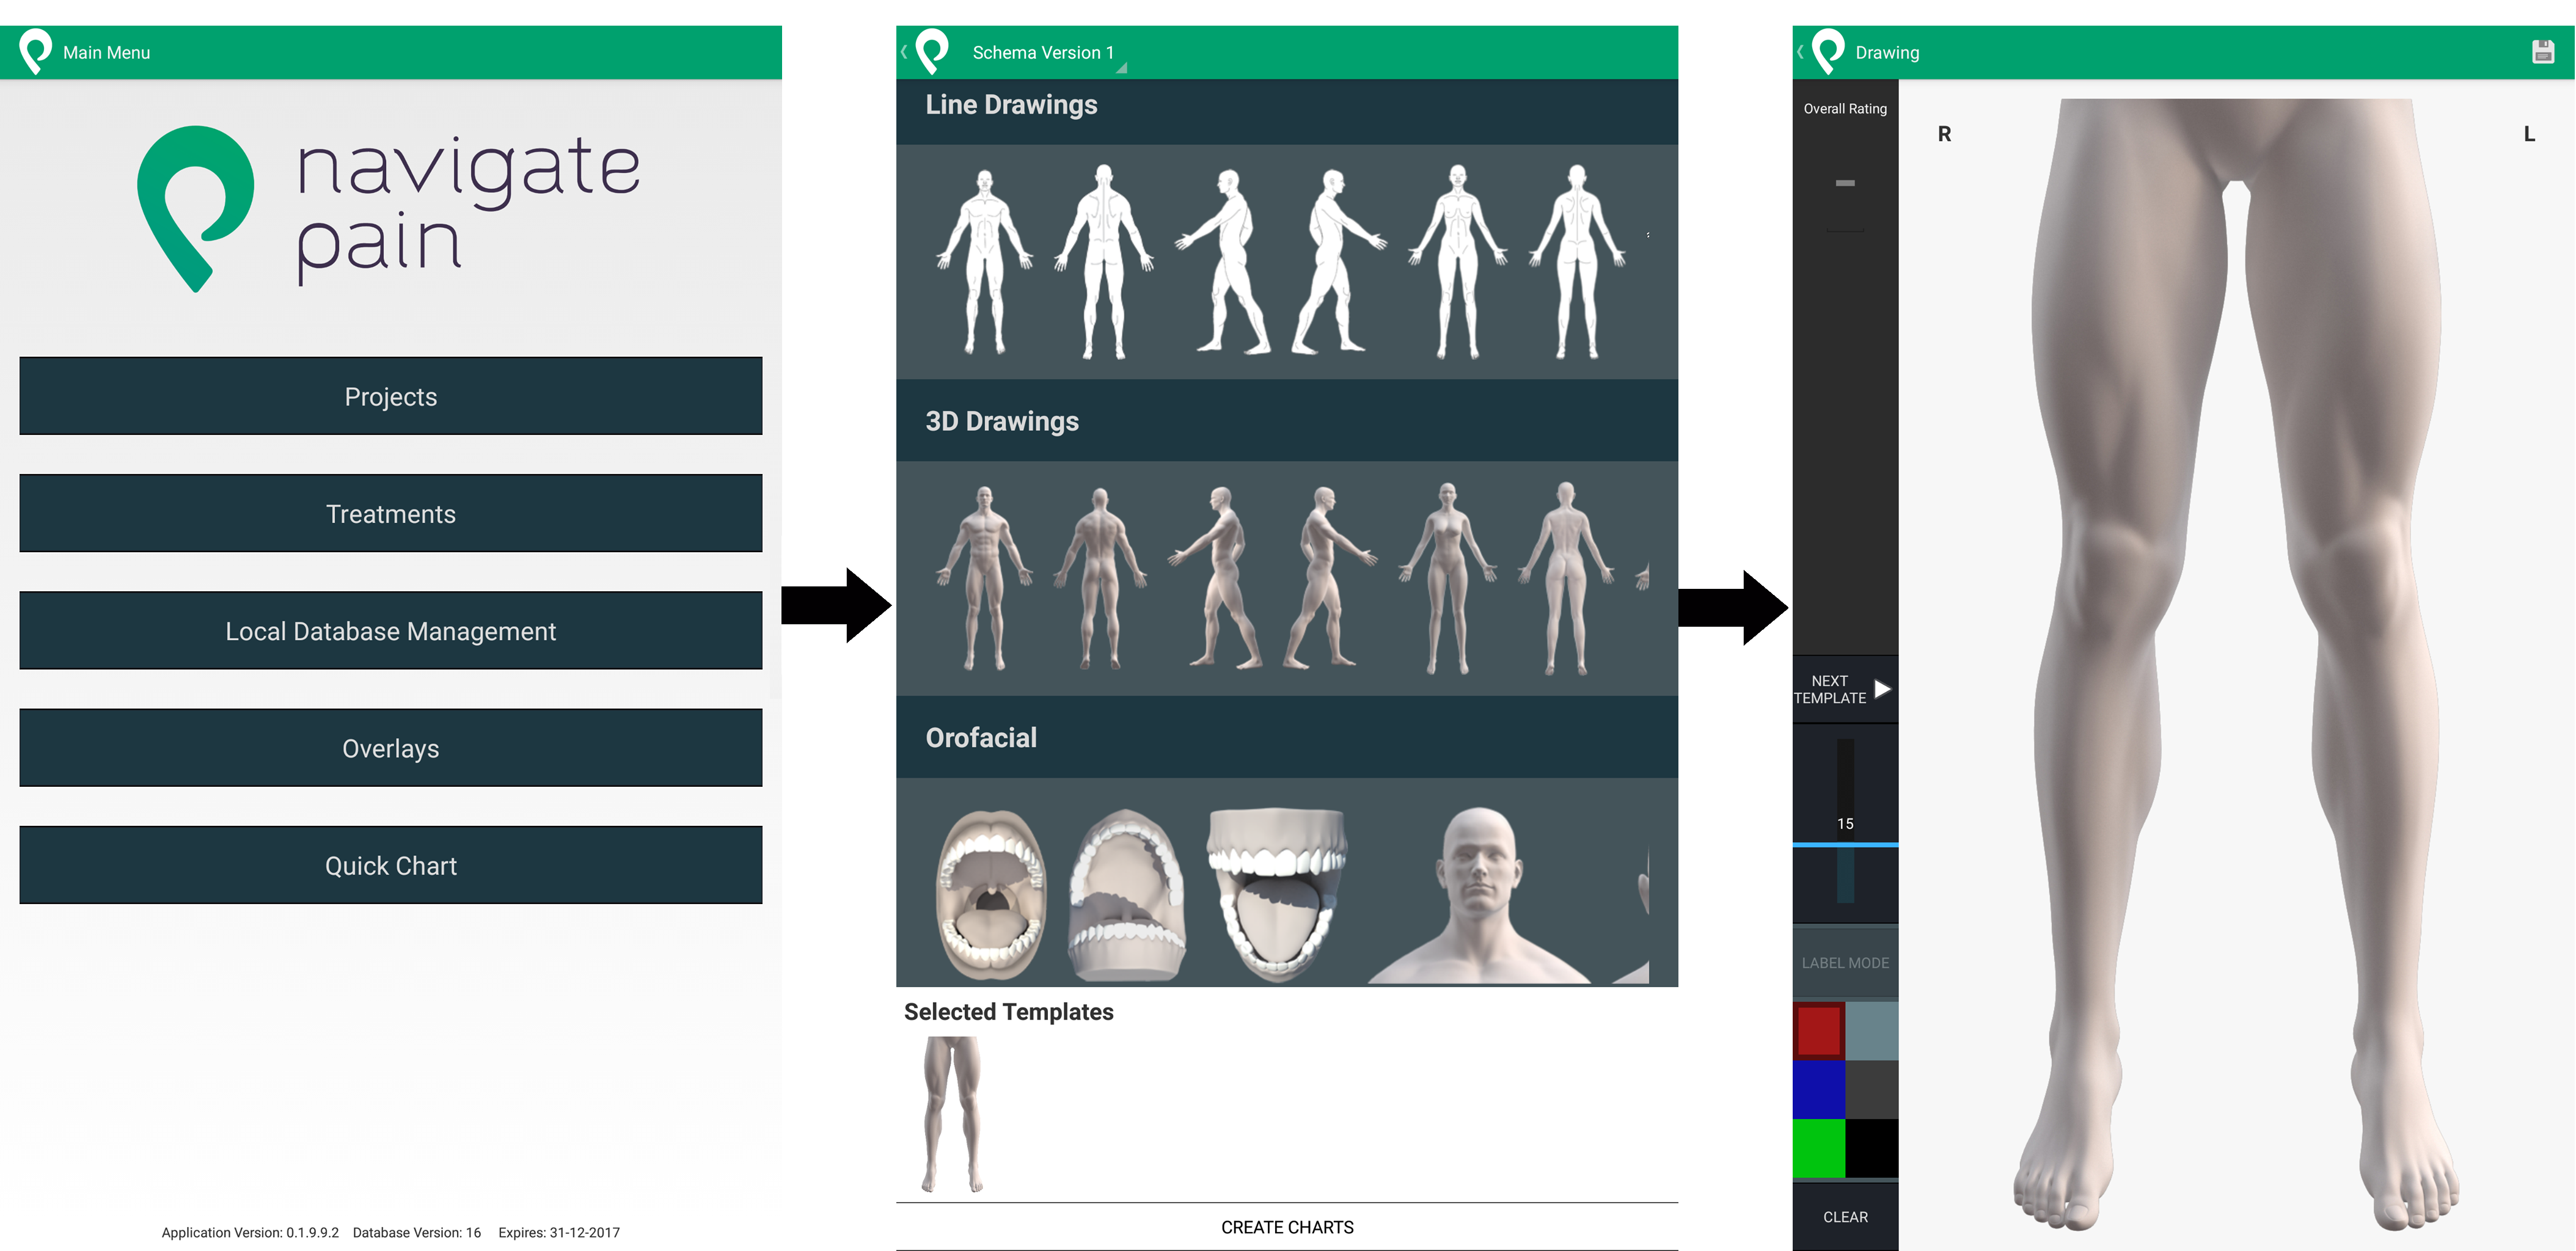
\includegraphics[width=1\textwidth]{figures/Navigatepain}
\caption{The figure illustrates the process for making a pain map with Navigate Pain. There is three screenshots of the application.}
\label{fig:Navigatepain}
\end{figure}

\noindent
The left screen in figure \ref{fig:Navigatepain} is the main screen. By clicking on "Project" a folder with subjects is created. From each subject information like name, age, height is saved. Before the subject can draw their pain areas, the body outline has to be chosen, which illustrates the screen in the middle. The body outlines is divided into five categories: Line Drawings, 3D Drawings, Orofacial, Special Zooms and Knee Pain. In the bottom the seleceted templates is shown. When clicking on "CREATE CHARTS" the right screen is shown. Here it is possible to draw the pain areas with different colors and line thickness, which can be seen in the left side of the screen. Afterwards the pain map can be saved. 


\subsection{Data representations}
It is presumed that different data representations of pain maps affect the performance
accuracy of a deep learning model, which is why different data representations are created. 
A study found a correlation between a prolonged symptom duration and the size of the pain area. It was shown that the pain area increased for individuals that have a symptom duration for more than five years compared to those with a symptom duration below five years. Likewise pain intensity had a correlation with the size of pain area for symptom duration above five years. Furthermore, the shape of the pain developed from a U-shape to an O-shape for individuals with a symptom duration above five years.\citep{Boudreau2017} Based on this study the morphology is considered to be relevant to investigate, which is why morphology is one of the data representations.\\

\noindent
The PFP is often described as diffuse pain and therefore difficult to describe and localise \citep{Witvrouw2014}. To accommodate this is it chosen to divide the pain into different knee regions, which may indicate whether a specific region of the knee influence the PFP. This is converted to a simplified data representation that indicate active knee regions. 
A combination of the two data representation is combined to create a third data representation which both include the morphology of the pain and the different knee regions. 
Gender is included as an input parameter in the three data representations, because it is shown that the prevalence is more than twice as high for females than males \citep{Petersen2013, Rathleff2015}.  

\noindent
Since the symptom duration of PFP seems to affect the size and shape of the pain area, is it chosen to classify the three data representations in proportion to symptom duration. Likewise is it chosen to classify pain intensity because of the influence from the size of pain area.
The three data representations is referred to as morphology-representation, regions-representation and superimposed-representation.


\section{Pre-analysis}
The pain maps and associated symptom duration and pain intensity are analysed to get an overview of the data. The data is analysed in MatLab, where the distribution of the outputs, symptom duration and pain intensity, are investigated whereafter the classifications to the neural network models are decided. Furthermore the distribution of gender is compared to the literature which states that the prevalence is higher for females than males.
To select the threshold for data representation according to the active pain regions are the pain areas in different pain maps analysed. 
Simple linear regressions of pain area and either symptom duration or pain intensity are made to get a reference to the neural network models. 

\subsection{Classification of data}
The neural networks models have to classify the data representations into categories. To find these are histograms of the outputs created. \\

\noindent
A histogram of the symptom duration associated with the pain maps is illustrated in figure \ref{fig:histoduration}.

\begin{figure} [H]
\centering
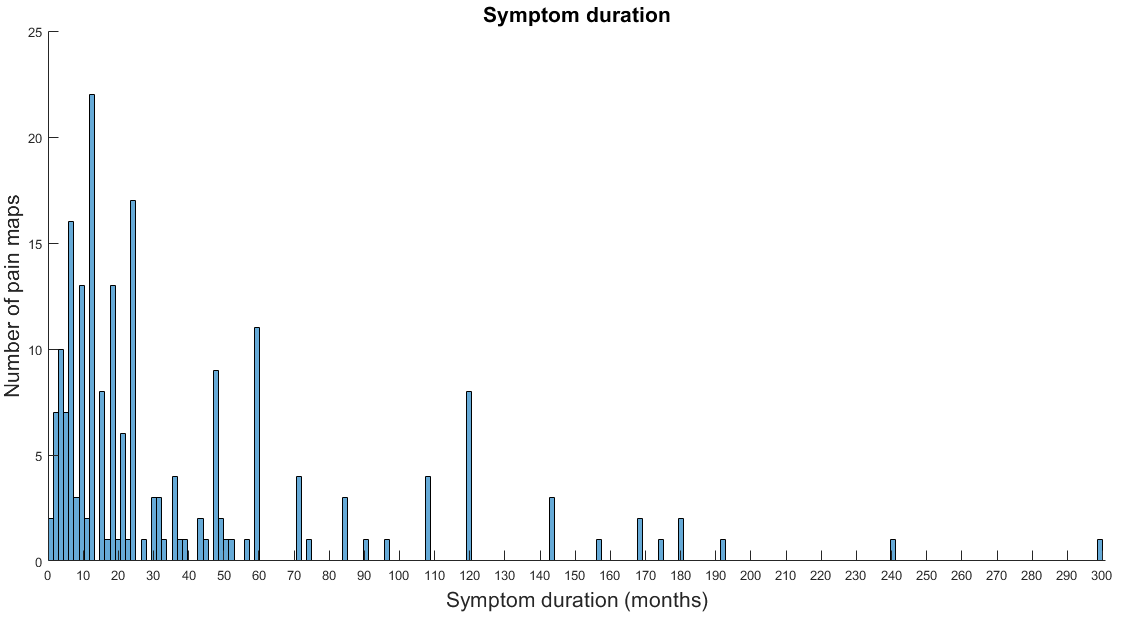
\includegraphics[width=1\textwidth]{figures/histogramDuration}
\caption{A histogram of the symptom duration.}
\label{fig:histoduration}
\end{figure}

\noindent
SOMETHING
hvor mange klasser
hvor de skal splittes 


In the appurtenant data to the pain map the individuals have stated their pain intensity like the worst pain in the last 24 hours and the last 7 days. 
It is not assumably that the individuals have performed any PFP provoked activity in the last 24 hours before drawing their pain, therefore it is chosen to use the worst pain intensity in the last 7 days to get a more average worst pain intensity. 
To explore the difference between the individuals’ stated pain intensity in the last 7 days is a histogram created which can be seen in figure \ref{fig:histopain}.

\begin{figure} [H]
\centering
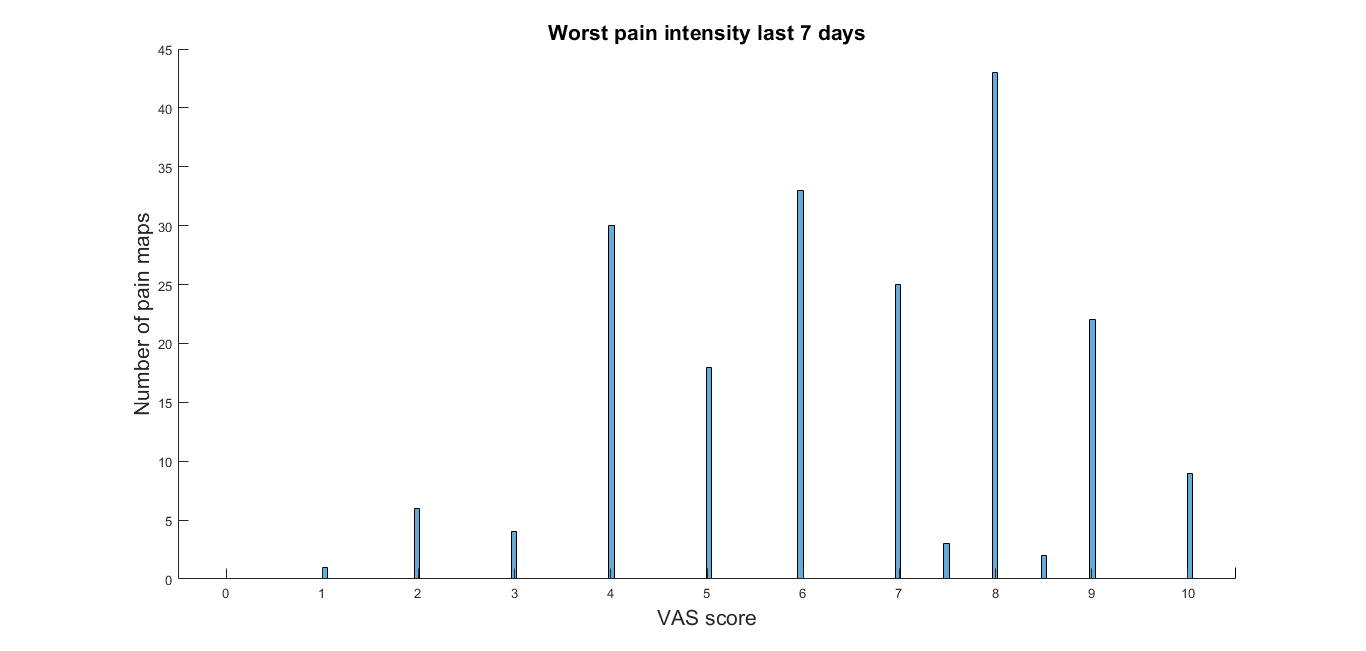
\includegraphics[width=1\textwidth]{figures/histrogramPain}
\caption{Histograms of the pain intensity the last 7 days.}
\label{fig:histopain}
\end{figure}

\noindent
The worst pain intensity is divided into some classes which the models should classify in addition to. To test the models are the data firstly divided into the extremes, since it is assumed that if the models predict badly with the extremes, the models would not predict better with multiple classification of the pain intensity. The extremes is chosen to be intervals 1 to 4 and 8 to 10 by which the last classification constitute the interval between. 


\subsection{Distribution and threshold}
Gender is an interesting parameter to use as an input, because the prevalence is more than twice as high for females than males. Thereto perceived pain is subjective and depends on the individual's character and personality. The distribution of gender is investigated by creating a histogram, which is shown in figure \ref{fig:histogender}. 

\begin{figure} [H]
\centering
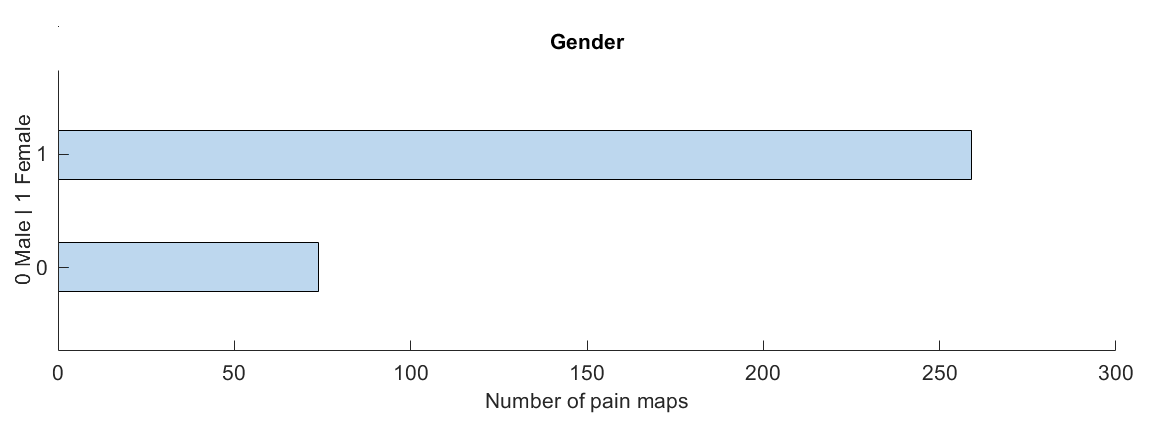
\includegraphics[width=1\textwidth]{figures/histoGender}
\caption{Histograms of the distribution/division of gender.}
\label{fig:histogender}
\end{figure}

\noindent
According to the given data the prevalence is higher for females than males. The females constitute 156 of the 206 individuals.

\noindent 
In relation to the data representation that contains information about the active pain regions, it is necessary to find a threshold that decides when a knee region contains enough pain pixels to be considered active. A threshold is required to increase the confidence of an active pain region by avoiding minimal contributions e.g. small pain areas in the associated regions. Simultaneous may the threshold not be too large so potential pain regions will not be incorporated. The threshold to indicate active pain regions is decided based on an analysis, where threshold values of 0, 5, 10 and 15 percent are tested. The analysis of the threshold is tested on five random pain maps to get a general impression of the data. To better illustrate the division of the pain regions are the regions in figure \ref{fig:atlas} colored in different colors that are easier to distinguish, which is shown in figure \ref{fig:colorregion}.

\begin{figure} [H]
\centering
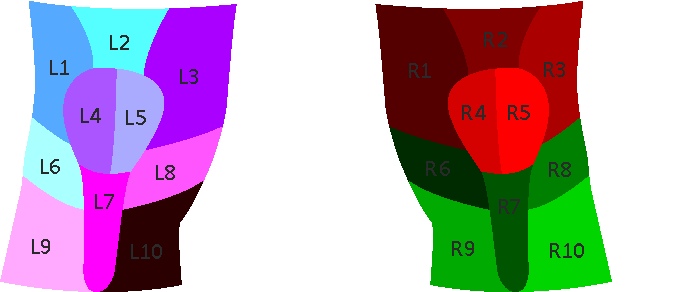
\includegraphics[width=0.7\textwidth]{figures/colorregion}
\caption{Knee regions colored in colors that are easier to distinguish.}
\label{fig:colorregion}
\end{figure}

\noindent
An example of pain maps and appurtenant bar chart are illustrated in figure \ref{fig:threshold}. The pain maps, figure \ref{threshold}(a-d), are likewise colored in the same colors as figure \ref{fig:colorregion} to indicate which regions that are affected according to 0, 5, 10 and 15 percent threshold. The last figure (e) is the bar chart that indicates how many and which active regions there are according to the threshold values.

\begin{figure} [H]
\centering
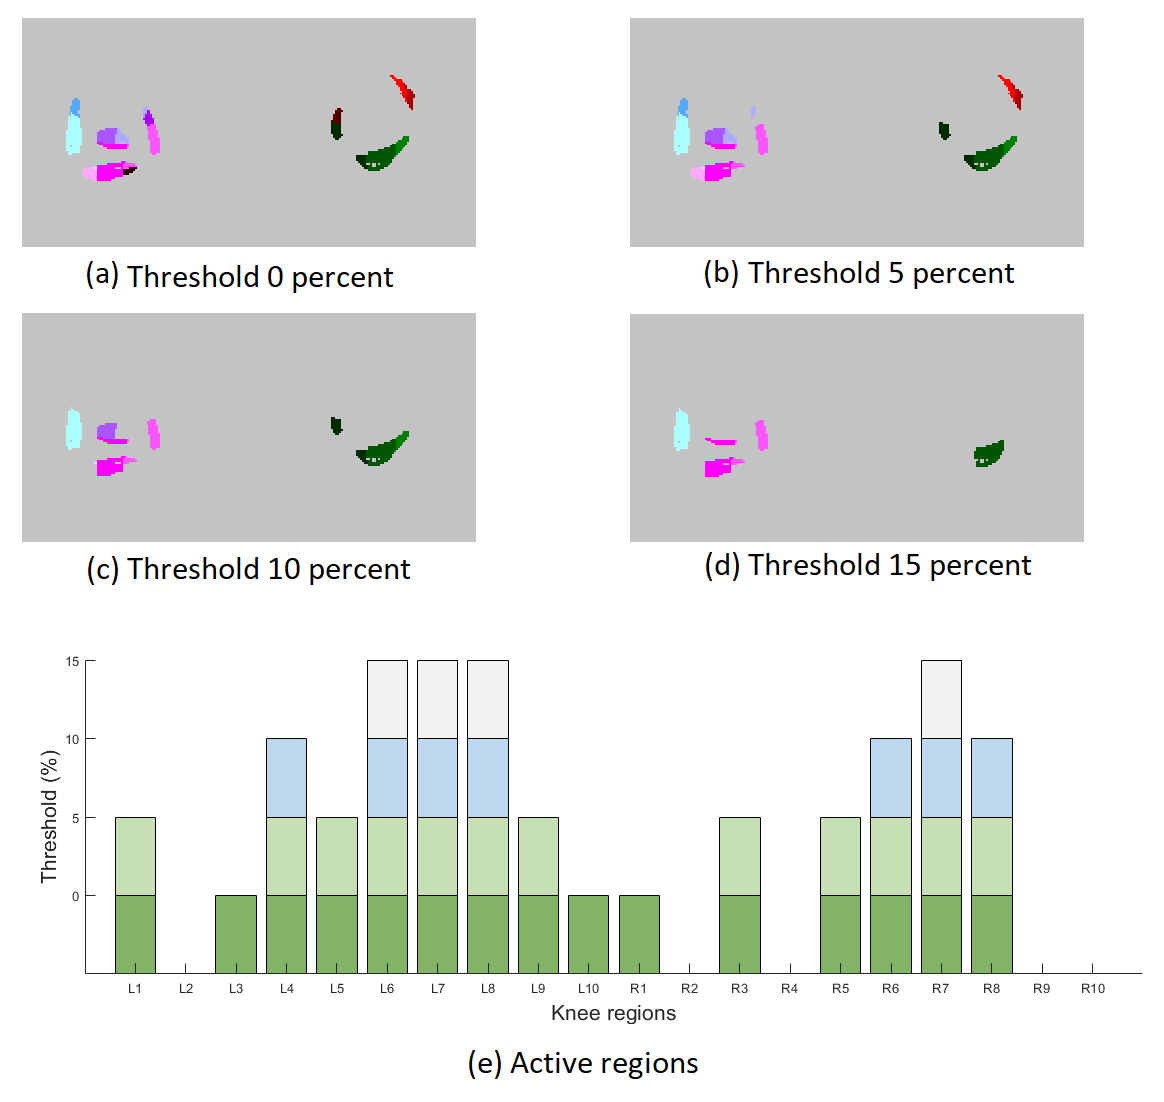
\includegraphics[width=1\textwidth]{figures/threshold4}
\caption{The active knee regions when the threshold is (a) 0 percent, (b) 5 percent, (c) 10 percent and (d) 15 percent. (e) is the bar chart that indicates how many and which knee regions that are considered active.}
\label{fig:threshold}
\end{figure}

\noindent
According to figure \ref{fig:threshold} (a) and (e) is it shown that the knee to the left has nine active regions and the knee to the right has six active knee regions, when the threshold is zero. In proportion to the active regions are region L3, L10 and R1 very small and are thereby the first regions to be discarded when the threshold is increased by five percent, which is shown in figure (b). 
By comparison figure (a) and (b) are there minor changes according to the missing regions, compared to figure (c) and (d) where greater areas disappears after increasing the threshold to 10 and 15 percent. 

Based on analysis of the five pain maps and bar charts, figure \ref{fig:threshold4} and appendix \ref{app:XX}, is a threshold on five percent chosen to avoid including minor pain areas, like L10, as active knee regions, and to avoid discarding too many and large areas, like R3 and R5.


\subsection{Simple regression models}
To test whether there is a linear correlation between the size of the pain area and the symptom duration and pain intensity, are simple regression models made. If the size can predict the symptom duration and pain intensity, it may not be significant to investigate pain morphology and location.

In figure \ref{fig:durationRegression} is a linear regression fit of symptom duration and size of pain area illustrated. 

\begin{figure} [H]
\centering
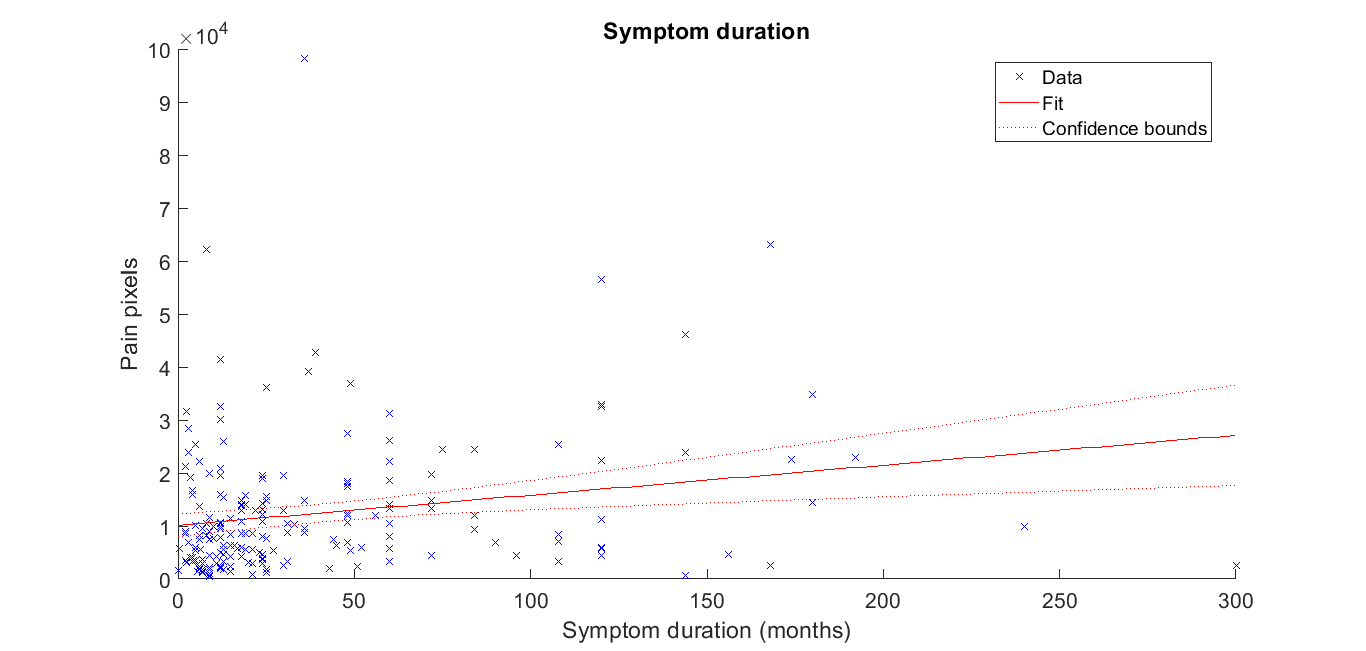
\includegraphics[width=1\textwidth]{figures/durationRegression}
\caption{A simple linear regression fit of symptom duration and the size of pain area.}
\label{fig:durationRegression}
\end{figure}

\noindent
The linear regression model of symptom duration has an R-squared value of 0.046, which is close to zero and therefore the model is not a good fit for the data. 
A linear regression model of pain intensity and the size of pain area is also made, which is illustrated in figure \ref{fig:painRegression}.

\begin{figure} [H]
\centering
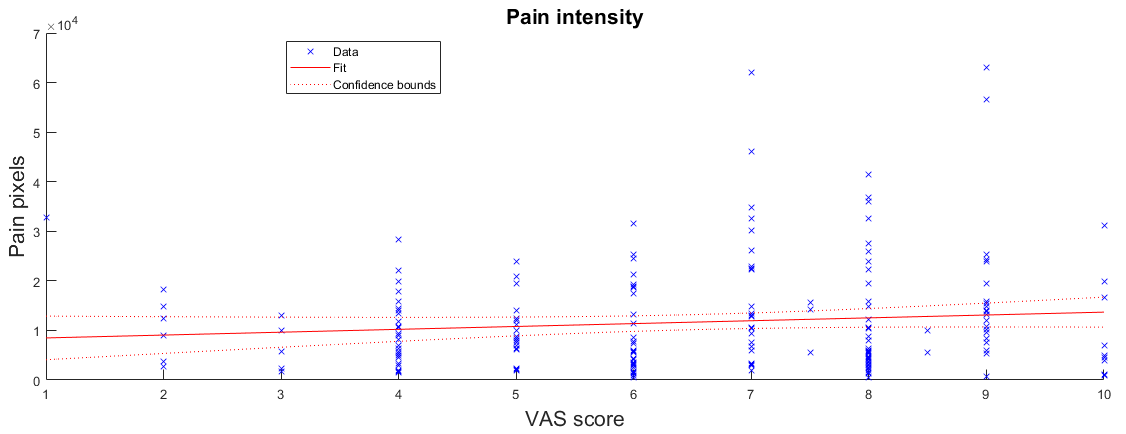
\includegraphics[width=1\textwidth]{figures/painRegression}
\caption{A simple linear regression fit of pain intensity and the size of pain area.}
\label{fig:painRegression}
\end{figure}

\noindent
The R-squared value of this model is 0.0117, so the linear model is not a good fit on the data. 
These linear regression models are not very suitable when trying to predict symptom duration or pain intensity from the size of pain area. However they can be compared to the performance of the neural network models.  



\section{Pre-processing}
The data is pre-processed in MatLab to prepare it to the three different neural network models. Each model has an appurtenant data representation which are prepared in three different ways. The three data representations are morphology, regions and superimposed morphology and region. Common for the data representation is that the pain maps are imported as image-matrices whereafter the matrices are resized, since the given data was collected at different resolutions (screen sizes). Furthermore, the matrices are cropped to sort out unnecessary data like the areas inferior and superior to the knee.
Before the data is used as an input in the neural network models, the image-matrices are converted into vectors whereafter they are assembled in one matrix for each data representation. To get additional information associated with the pain maps, is gender added by including a column vector to the three matrices. 
In addition to the input, the neural network models need an output to train the models. The output, which is either symptom duration or pain intensity, is likewise added as a column vector. 
The following sections describe the pre-processing of the individual data representations. 

\subsection{Morphology-representation} \label{sec:Morph}
The first representation of data is a binary matrix of the original pain maps.
Firstly, the image of the original pain map is gray-scaled to get a one-dimensional matrix instead of a three-dimensional RGB-matrix. This matrix is then converted into a matrix consisting of zeroes and ones, where the pain pixels are symbolized with ones. An original pain map and a pain map consisting of a binary matrix is shown in figure \ref{fig:cropbin7}.

\begin{figure} [H]
\centering
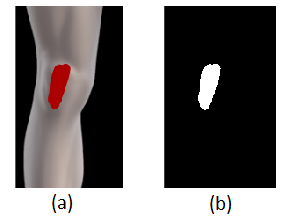
\includegraphics[width=0.7\textwidth]{figures/cropbin7}
\caption{(a) Original pain map and (b) image consisting of a binary matrix where white color represents the pain pixels.}
\label{fig:cropbin7}
\end{figure}

\noindent
An illustration of this data representation is created to convey how the data is assembled and transferred to the model. The illustration is shown in figure \ref{fig:binmatrix}.

\begin{figure} [H]
\centering
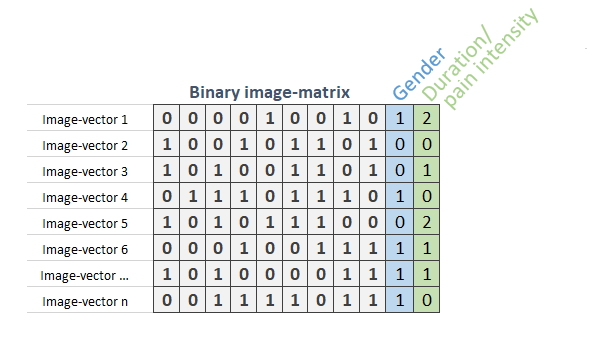
\includegraphics[width=0.8\textwidth]{figures/binaryimagematrix}
\caption{An illustration of the matrix of the morphology data representation. The matrix consist of image-vectors for each subjects where the two last column indicate the appurtenant gender and either duration or pain intensity. The image-vectors has a length equal to the number of pixel in the pain maps.}
\label{fig:binmatrix}
\end{figure}


\subsection{Regions-representation}
The second representation of the data is a matrix consisting of vectors with 20 values which indicate pain in relation to the knee regions.
The knee regions shown in figure \ref{fig:atlas} are converted into a matrix consisting of 20 values, which represent each knee regions. This matrix is superimposed to the binary image of the pain map, which results in a matrix with pain represented in each knee region. In figure \ref{fig:binregions} are the knee regions and the pain associated with the regions illustrated.

\begin{figure} [H]
\centering
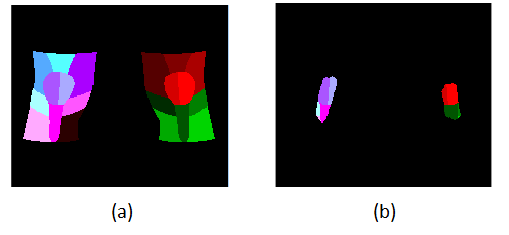
\includegraphics[width=0.8\textwidth]{figures/binregions}
\caption{(a) Knee regions and (b) pain in the specific regions.}
\label{fig:binregions}
\end{figure}

\noindent
After superimposing the two matrices, knee regions and pain, the number of pixels in each active knee region is found. This number is compared to the total number of pixels that are in each knee region, so knee regions with less than 15 \% pain are excluded. WHY 15\%. As a result a vector with 20 values is created. This data representation is implemented the same way as the first representation, figure \ref{fig:binmatrix}. The only difference is that the length of the image-vectors respond to the 20 regions, and therefore are there only 20 values in this data representation.


\subsection{Superimposed-representation}
The third representation of the data is a matrix consisting of individuals’ pain divided into the knee regions.
\noindent
In this representation the superimposed matrix from the second data representation is used. Since the data representation should reflect the morphology of the pain and divide the pain into the different knee regions is one-hot encoding used. One-hot encoding is a way to separate categorical data into binary data \citep{Harris2012}. This means that the 20 values for each knee region do not have a correlation. After one-hot encoding the superimposed matrix consists of 20 layers where each layer represents a knee region. An illustration of this data representation is shown in figure \ref{fig:onehot}.


\begin{figure} [H]
\centering
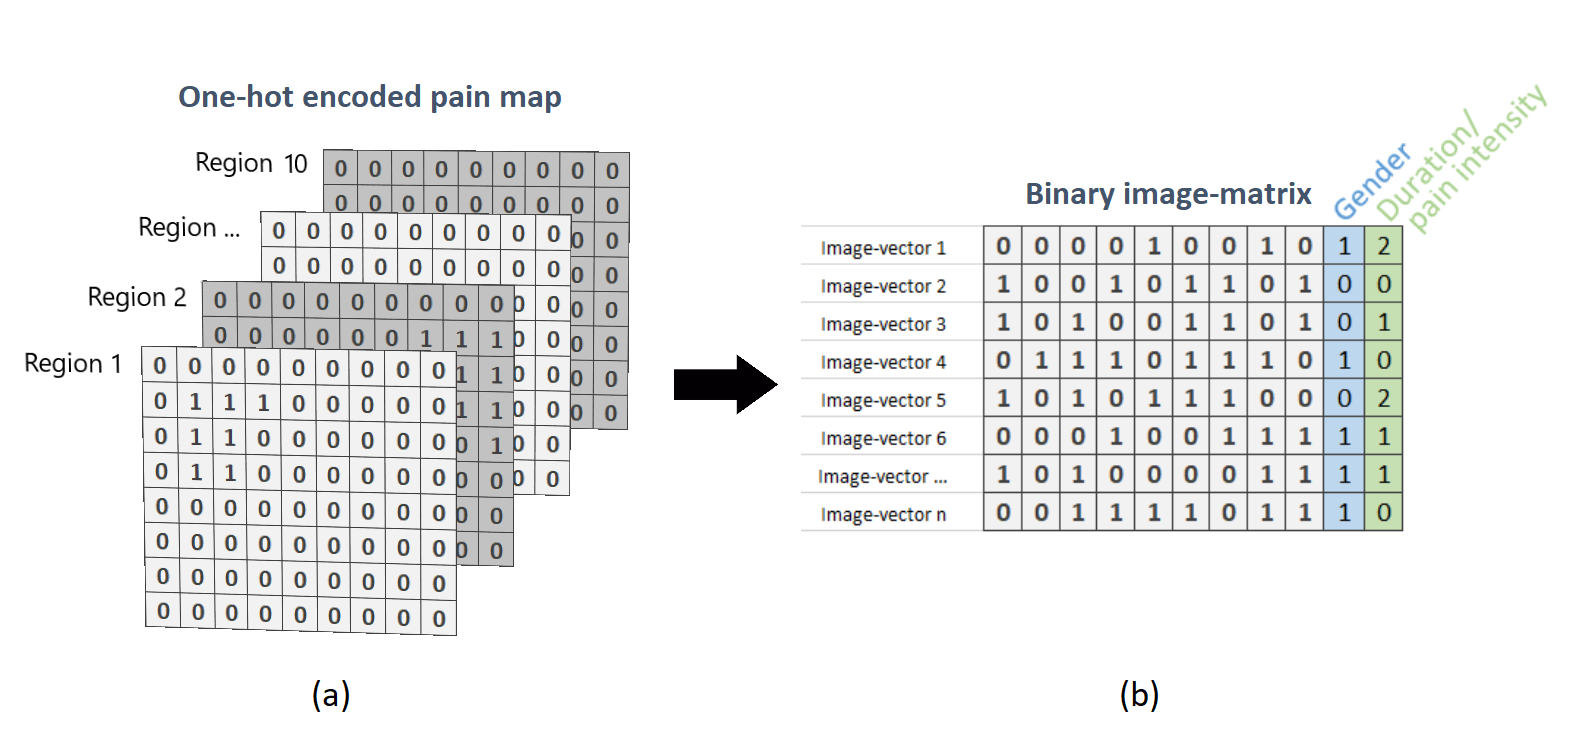
\includegraphics[width=1\textwidth]{figures/onehotmatrix}
\caption{(a) illstrates the one-hot encoded pain map and (b) shows the images-vectors in one assembled matrix with gender and either symptom duration or pain intensity.}
\label{fig:onehot}
\end{figure}